\section{Architettura Event-driven}

\section{Tecnologie utilizzate}

L'applicativo si basa su tecnologie e servizi ampiamente adottati e consolidati in ambiente aziendale:

\subsection{RabbitMQ}
Rabbit\footnote{Questa sezione utilizza informazioni tratte dalla documentazione ufficiale di RabbitMQ\cite{rabbitmq}}
\`e un message broker, cio\`e, un software che consente la comunicazione asincrona tra programmi.
Funziona attraverso \textbf{queues} (code) su cui i \textbf{producers} (mittenti) inviano messaggi definiti a priori,
e i \textbf{consumers} (destinatari) consumano questi messaggi eseguendo operazioni in base al loro contenuto.
Rabbit in particolare utilizza gli \textbf{exchange}, un punto intermedio tra i producers e le queues.
L'exchange riceve i messaggi dei producers e li instrada confrontando la \textbf{routing key} del messaggio con determinate regole dette \textbf{bindings}.
\\\\
Rabbit ha diversi punti di forza, alcuni intrinsechi del tipo di software di cui fa parte, altri per via delle sue caratteristiche specifiche:\
\begin{itemize}
  \item \textbf{Scalabilit\`a} -  Il carico di lavoro viene distribuito automaticamente tra i consumers, e finch\'e i messaggi
    non vengono processati questi rimangono in coda.
  \item \textbf{Flessibilit\`a nel routing dei messaggi} - Rabbit offre molteplici modi di configurare gli exchange a seconda delle esigenze:
    \begin{enumerate}
      \item \textbf{Direct Exchange} - Invio dei messaggi a code specifiche in base a una routing key.
        \begin{figure}[H]
          \centering
          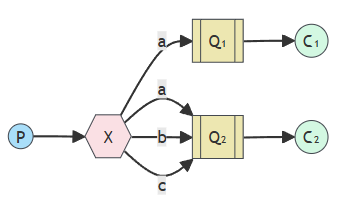
\includegraphics[width=5cm]{images/rabbitmq-direct-exchange.png}
          \caption{Esempio di Direct Exchange\cite{rabbitmq}}
        \end{figure}
      \item \textbf{Fanout Exchange} - Invio su tutte le code appartenenti all'exchange, utile per il broadcasting.
      \item \textbf{Topic Exchange} - Permette di instradare i messaggi facendo il match delle routing key con binding basati su pattern pi\`u o meno complessi.
        \begin{figure}[H]
          \centering
          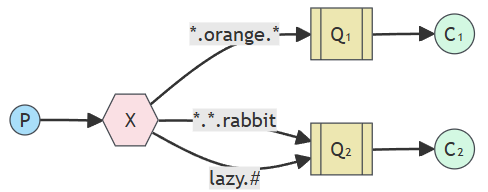
\includegraphics[width=7cm]{images/rabbitmq-topic-exchange.png}
          \caption{Esempio di Topic Exchange\cite{rabbitmq}}
        \end{figure}
      \item \textbf{Header Exchange} - Utile per instradare i messaggi in base a molteplici argomenti, per esempio \`e possibile creare una coda
        che riceve solo messaggi con header ``format=pdf''.
    \end{enumerate}
  \item \textbf{Affidabilit\`a} -  Rabbit \`e in grado di offrire un elevato grado di affidabilit\`a grazie a  molteplici meccanismi:
    \begin{enumerate}
      \item
        \textbf{Acknowledgements} -  Una conferma da parte del consumer che tutto sia andato a buon fine.
        Se il consumer non invia l'ack, Rabbit terr\`a il messaggio all'interno della coda o lo invier\`a ad un altro consumer.
      \item \textbf{TTL (Time-to-Live) per messaggi e code} - \`E possibile impostare un limite di tempo che un messaggio pu\`o rimanere
        in una queue, dopo il quale vengono automaticamente scartati o vengono spostati su un DLX, riducendo il rischio che si
        possano accumulare messaggi causando problemi di risorse esaurite o code sovraccariche.
      \item \textbf{DLX (Dead-letter Exchange)} - Sono normali exchange su cui vengono inviati i messaggi \textbf{``dead-lettered''}: messaggi che hanno
        ricevuto un nack (\textbf{negative acknowledgement}), messaggi che hanno superato il TTL definito per messaggio, messaggi
        scartati perch\`e la queue ha superato uno dei limiti imposti, o messaggi che hanno superato il numero massimo di re-try consentito dalla coda.
      \item \textbf{Persistenza dei messaggi} -  \`E possibile persistere i messaggi presenti nelle queue sul disco,
        cio\`e non vengono persi al riavvio o al crash del server. La persistenza pu\`o essere attivata sia sulle code che sui singoli messaggi.
        Il contro della persistenza \`e che aumenta la latenza, ma offre ovviamente una maggiore affidabilit\`a.
    \end{enumerate}
\end{itemize}

\subsection{PostgreSQL}
La scelta di PostgreSQL deriva dalla completezza delle funzionalit\`a che offre, che lo rendono un'opzione desiderabile per applicazioni aziendali.
Di seguito alcune delle caratteristiche che lo contraddistinguono:

\begin{itemize}
  \item \textbf{Elevate prestazioni} - \`E un database relazionale molto performante in grado di supportare decine di migliaia di operazioni al secondo sul giusto hardware,
    e offre una latenza minore rispetto a DBMS concorrenti come \textbf{MySQL} in molte operazioni.\cite{salunke2024performance}
  \item \textbf{Robustezza} - Postgres supporta molte funzioni di sicurezza, come autenticazione SSL, o configurazione dei permessi granulare fino al
    livello di colonne e righe.
    \`E inoltre completamente conforme ai requisiti \textbf{ACID} (Atomicity, Consistency, Integrity, Durability).
    Per assicurare queste propriet\`a, PostgreSQL utilizza metodologie come \textbf{Multi-Version Concurrency Control} (MVCC) e \textbf{Write-Ahead Logging} (WAL).
  \item \textbf{Scalabilit\`a} - Ha ottime capacit\`a di scalabilit\`a verticale, che si traduce nell'utilizzo di tutti i core,
    di tutta la RAM o di maggiore velocit\`a di lettura/scrittura dei dischi.
    Supporta inoltre il clustering e la replication, e ha quindi anche capacit\`a di scalabilit\`a orizzontale.
    \begin{figure}[H]
      \centering
      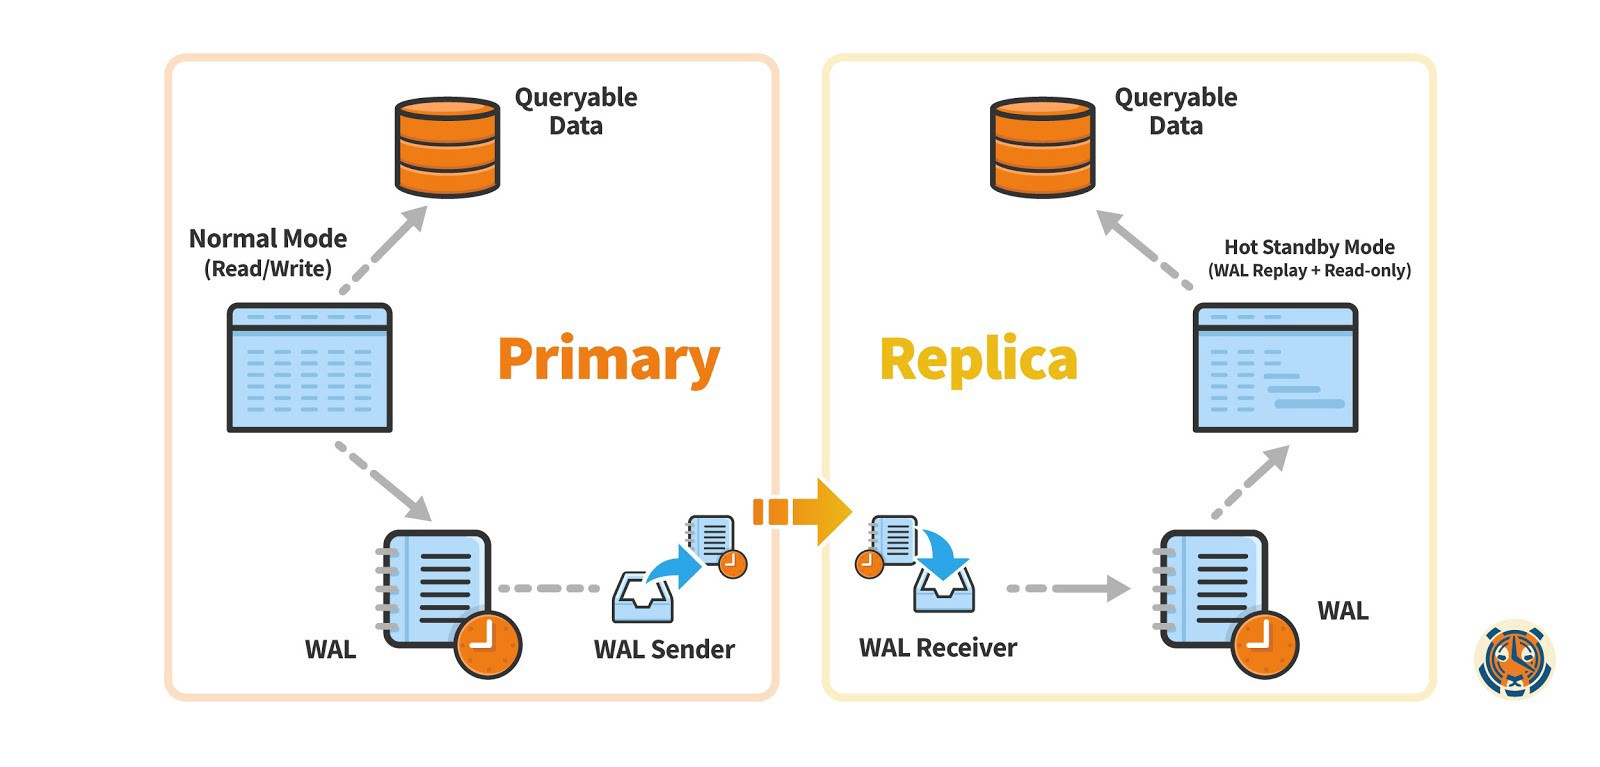
\includegraphics[width=15cm]{images/postgres-replication.png}
      \caption{Esempio di replica\cite{postgreshighavail}}
    \end{figure}
  \item \textbf{Supporto per transazioni complesse} - Postgres supporta la scrittura di transazioni complesse e funzioni procedurali attraverso un linguaggio chiamato
    \textbf{PL/pgSQL}, che permette di creare logiche pi\`u avanzate.
\end{itemize}
\subsection {Spring e SpringBoot}
Spring \`e un framework di Java creato per semplificare lo sviluppo di applicazioni a livello enterprise, fornendo una serie di strumenti per gestire i problemi pi\`u comuni
durante lo sviluppo, permettendo agli sviluppatori di concentrarsi sulla business logic piuttosto che sui dettagli implementativi.
Esempi di questi sono Spring Data o Spring Security.

Spring si basa sul concetto di \textbf{Inversion of Control} (IoC), dove gli oggetti invece di creare le loro dipendenze direttamente le ricevono da fonti esterne.
Questo \`e implementato attraverso un pattern chiamato \textbf{Dependency Injection}, in cui gli oggetti definiscono le proprie dipendenze e lo \textbf{Spring IoC Container}
gliele fornisce quando vengono creati.
Lo Spring IoC Container si occupa dell'intero ciclo di vita di un oggetto, e nel contesto di Spring questi prendono il nome di \textbf{bean}.
\\\\
Spring da solo \`e difficile da configurare e richiede molto boilerplate. Per cercare di ovviare a questo problema \`e stato creato il progetto \textbf{SpringBoot}.
Lo scopo di SpringBoot \`e quello di semplificare il processo di configurazione di Spring, configurando automaticamente le dipendenze incluse in modo ragionevole.
Per esempio, se si volesse utilizzare un web-server, basta includere spring-boot-starter-web tra le dipendenze e SpringBoot configurer\`a automaticamente un web-server come Tomcat, di default.
\subsection{Angular}
Angular è un framework JavaScript creato da Google e ideato per creare \textbf{Single-Page Web Applications} (SPA). È profondamente integrato con TypeScript,
che significa avere una serie di vantaggi come maggiore Type Safety, codice più leggibile e mantenibile, oltre ad avere maggiori aiuti da IDE moderni come Visual Studio Code
con l'autocompletamento. Angular fornisce un pacchetto ben fornito di funzionalità anche senza l'utilizzo di librerie aggiuntive, tra cui ottimi strumenti di gestione del
routing, gestione dei form, client HTTP, gestione dello stato, integrazione nativa con RxJS e altro.

Per il progetto Sentinel inoltre è stato scelto di usare il \textbf{SignalStore di NgRx}, una soluzione di gestione dello stato completamente basata sui \textbf{Signal} di Angular,
introdotti in developer preview in Angular 16. Nei capitoli successivi verrà discussa più in dettaglio l'implementazione delle feature per la gestione di uno stato
con chiamate ad un server.
\subsection{Stripe}
Stripe \`e una piattaforma di pagamento che funge da intermediario nelle transazioni elettroniche.
%TODO Scrivere un'introduzione decente
% Prezzo per transazione: \texteuro 0,25 + 1.5\% per ogni transazione eseguita con carte europee.

\begin{itemize}
  \item \textbf{Facilit\`a di integrazione} - Il processo di integrazione all'interno di un applicativo \`e semplice, e offre molte opzioni di configurazione e servizi.
    A seconda delle esigenze, \`e possibile passare da una configurazione predefinita con zero o comunque pochissimo codice a un'esperienza completamente personalizzata dallo sviluppatore.
  \item \textbf{Sicurezza} - Stripe semplifica l'oneroso lavoro di integrare di un sistema di pagamenti che rispetta gli standard PCI DSS, essendo tutto gestito
    direttamente con redirect a Stripe o attraverso elementi integrati nell'applicazione ma hostati sui loro server. Non c'\`e quindi bisogno di trattare e memorizzare dati
    riguardanti i metodi di pagamento, evitando tutte le complicazioni che ne conseguono.
  \item \textbf{Supporto a molti metodi di pagamento} - Stripe supporta tutti i maggiori circuiti di pagamento, bonifici, o anche wallets digitali come Google Pay o Apple Pay.
  \item \textbf{Documentazione estensiva} - La documentazione \`e molto completa e dettagliata, inoltre \`e piena di esempi di integrazione in diversi linguaggi.
\end{itemize}
\subsection{Docker}
Docker\footnote{Questa sezione utilizza informazioni tratte dalla documentazione ufficiale di Docker\cite{dockerdocs}}
\`e uno dei software pi\`u popolari in ambito aziendale e non, per la sua capacit\`a di creare dei container dove vengono eseguite le applicazioni in maniera isolata.
Docker si basa su alcuni concetti fondamentali:
\begin{itemize}
  \item \textbf{Docker Images} - Sono dei template che vengono utilizzati per creare i container. Contengono tutte le configurazioni e gli eseguibili delle dipendenze richieste
    dall'applicazione containerizzata. Sono in genere molto leggere, visto che devono essere portabili. Le immagini possono essere condivise attraverso repository come Docker Hub.
  \item \textbf{Docker Containers} - L'ambiente dove l'applicativo containerizzato viene eseguito. Nel caso di un sistema Linux, al contrario di un normale software di virtualizzazione
    i container di Docker vengono eseguiti sullo stesso kernel del sistema host. Questo significa che se un'applicazione containerizzata richiede una system call specifica
    per venire eseguita e la versione del kernel installata sull'host non la supporta, non \`e possibile eseguire quel container. Su Windows e macOS invece viene eseguito
    attraverso una VM Linux, in quanto \`e necessario un kernel Linux per utilizzare Docker.
  \item \textbf{Dockerfile} - Un file di testo che contiene tutte le istruzioni necessarie per creare un'immagine. Al suo interno viene specificata una \textbf{base image},
    un'immagine che la build andr\`a ad estendere. \`E possibile anche creare un'immagine da zero, ed \`e possibile utilizzare immagini diverse per buildare l'applicazione e per eseguirla
    (\textbf{Multi-staged build}). Per esempio, \`e comune utilizzare un'immagine minimale di Linux come alpine per buildare un sito, per poi prendere il risultato e usarlo con
    l'immagine base di nginx,
  \item \textbf{Docker Compose} - Permette di definire applicazioni multi-container, offrendo opzioni come la possibilit\`a di specificare dipendenze tra container, variabili d'ambiente,
    mapping tra porte interne ed esterne al container, e creare dei network virtuali.
\end{itemize}

\subsection{Kubernetes}
Kubernetes\footnote{Questa sezione utilizza informazioni tratte dalla documentazione ufficiale di Kubernetes\cite{kubernetesdocs}}
\`e un \textbf{container orchestrator}, ovvero un software che si occupa di gestire automaticamente applicazioni containerizzate.
Funziona attraverso un'architettura master-worker. Un \textbf{master node} si occupa di coordinare tutte le attivit\`a, mentre i \textbf{worker node} si occupano di eseguire i container.
\\\\
L'unit\`a pi\`u piccola creabile e deployabile \`e un \textbf{pod}, un gruppo di container strettamente correlati che condividono lo stesso namespace.
\\\\
Kubernetes gestisce i pod attraverso quattro tipi di controller:
\begin{itemize}
  \item \textbf{Deployment} - Viene utilizzato nel caso sia necessario avere uno o pi\`u pod identici (\textbf{ReplicaSet}) che non devono mantenere uno stato persistente. Kubernetes si occupa
    di garantire che lo stato specificato nella configurazione venga rispettato, monitorando la salute dei pod e riavviandoli in caso di problemi.
    Un esempio di utilizzo \`e per hostare un web-server che restituisce contenuti statici.
  \item \textbf{StatefulSet} - Come un Deployment, gestiscono pod identici generati in base agli stessi container. La differenza \`e che l'identit\`a di ogni pod \`e unica e lo storage, cos\`i come l'identificativo di rete,
    vengono mantenuti in caso di rescheduling. Pu\`o essere utilizzato per applicazioni come database, o sistemi di caching (come Redis).
  \item \textbf{DaemonSet} - Vengono utilizzati per applicazioni che devono essere eseguite su ogni nodo, sono quindi utili per task come raccogliere log, monitoraggio o sistemi di rilevamento di intrusione.
  \item \textbf{Job} - Crea uno o pi\`u pod che continuano a venire eseguiti finch\'e un numero specifico di questi riesce ad arrivare a compimento. \`E possibile anche schedulare l'avvio di
    una task usando i CronJob.
\end{itemize}
Uno dei punti di forza pi\`u grandi di Kubernetes \`e la sua funzione di \textbf{Horizontal Pod Autoscaling}, che permette di regolare automaticamente il numero di pod avviati in base a
metriche di utilizzo delle risorse, rendendo semplice scalare automaticamente l'applicazione in base al carico.
